% --------------------------------------------------------------
% This is all preamble stuff that you don't have to worry about.
% Head down to where it says "Start here"
% --------------------------------------------------------------
 
\documentclass[12pt]{article}

\usepackage[margin=1in]{geometry} 
\usepackage{amsmath,amsthm,amssymb}
\usepackage[margin=1in]{geometry} 
\usepackage{amsmath,amsthm,amssymb}
%\usepackage[spanish]{babel} %Castellanización
\usepackage[T1]{fontenc} %escribe lo del teclado
\usepackage{inputenc} %Reconoce algunos símbolos
\usepackage{lmodern} %optimiza algunas fuentes
\usepackage{graphicx}
\graphicspath{ {images/} }
\usepackage{hyperref} % Uso de links

% To Display Chinese words
\usepackage{xeCJK}
% To Display Code
% \usepackage{listings}
\usepackage{minted}
% To Display csv file
\usepackage{csvsimple}
\usepackage{longtable}
\usepackage{booktabs}
 
\newcommand{\N}{\mathbb{N}}
\newcommand{\Z}{\mathbb{Z}}
 
\newenvironment{theorem}[2][Theorem]{\begin{trivlist}
\item[\hskip \labelsep {\bfseries #1}\hskip \labelsep {\bfseries #2.}]}{\end{trivlist}}
\newenvironment{lemma}[2][Lemma]{\begin{trivlist}
\item[\hskip \labelsep {\bfseries #1}\hskip \labelsep {\bfseries #2.}]}{\end{trivlist}}
\newenvironment{exercise}[2][Exercise]{\begin{trivlist}
\item[\hskip \labelsep {\bfseries #1}\hskip \labelsep {\bfseries #2.}]}{\end{trivlist}}
\newenvironment{problem}[2][Problem]{\begin{trivlist}
\item[\hskip \labelsep {\bfseries #1}\hskip \labelsep {\bfseries #2.}]}{\end{trivlist}}
\newenvironment{question}[2][Question]{\begin{trivlist}
\item[\hskip \labelsep {\bfseries #1}\hskip \labelsep {\bfseries #2.}]}{\end{trivlist}}
\newenvironment{corollary}[2][Corollary]{\begin{trivlist}
\item[\hskip \labelsep {\bfseries #1}\hskip \labelsep {\bfseries #2.}]}{\end{trivlist}}

\newenvironment{solution}{\begin{proof}[Solution]}{\end{proof}}

% write csv content in latex 
\begin{filecontents*}{grade.csv}
name,givenname,matriculation,gender,grade
Maier,Hans,12345,m,1.0
Huber,Anna,23456,f,2.3
Weisbaeck,Werner,34567,m,5.0
\end{filecontents*}
 
\begin{document}
 
% --------------------------------------------------------------
%                         Start here
% --------------------------------------------------------------
 
\title{2019 Deep Learning and Practice \\ Lab 6 -- InfoGAN}
\author{0756110 李東霖}

\maketitle
\section{Introduction}

DCGAN can generate hand-written digit image but it can't control generator to generate image with specific digit number. To solve that situation, need use InfoGAN to learn condition from noise.
\par \  \par
Lab's requirements as follows:

\begin{itemize}
\item Implement InfoGAN based on DCGAN (Deep Convolution GAN)
\item Show generated images
\item Plot loss curve of generator, discriminator, Q
\item Plot probability curve of read datas, fake datas before updating and fake datas after updating
\end{itemize}


\section{Experiment setup}

\subsection{Implement InfoGAN}

\subsubsection{Adversarial loss}

The GAN has two part. One is discriminator, another is generator. Discriminator classify images $x$ into real image and fake image. Generator yields image $x$ from noise $z$. 

\par \ \par
The loss of discriminator as follows:

\begin{equation}
\label{lossd}
    \text{loss}_D = -E_{x\sim P_{data}(x) }(\log D(x;\theta_D)) - E_{z\sim P_{z}(z)}(\log(1 - D(G(z; \theta_G); \theta_D)))
\end{equation}

The loss of generator has two options as follows:

\begin{align}
\label{lossg_1}
    \text{loss}_G & = -\text{loss}_D \\
\label{lossg_2}
    & = -E_{z\sim P_z(z)}(\log D(G(z; \theta_G); \theta_D) )
\end{align}

If loss equation of discriminator (\ref{lossg_1}) goes down, it means fake images from generator are more similar as real. But $\log (1 - D(G(z; \theta_G); \theta_D))$ in equation \ref{lossg_1} will lead to small gradient and slow convergence in generator. Because $D(G(z))$ usually is zero in early epoch and gradient near by zero is smaller than gradient near by one.

\begin{figure}[H]
\centering
% \includegraphics[width=\linewidth]{path/to/image} 
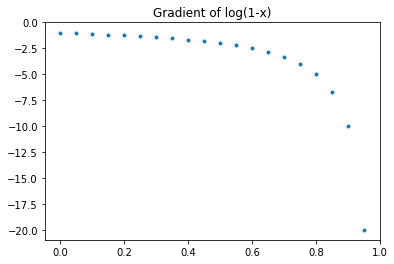
\includegraphics[width=\linewidth]{Images/gradientlog.png}
\caption{Gradient of log(1 - x)}
\end{figure}

Therefore, I chose equation \ref{lossg_2} to train InfoGAN. Equation \ref{lossg_2} converts disadvantage as advantage with gradient of $log(x)$ and zero $D(G(z)$ in begin.

\begin{figure}[H]
\centering
% \includegraphics[width=\linewidth]{path/to/image} 
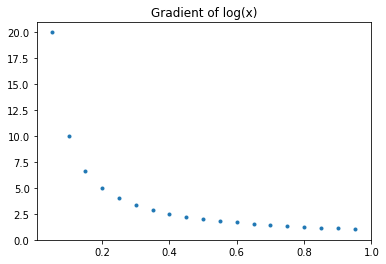
\includegraphics[width=\linewidth]{Images/gradientlog2.png}
\caption{Gradient of log(1 - x)}
\end{figure}

Implement of loss from equation (\ref{lossd}) as follows:

\begin{minted}[frame=lines, breaklines]{python}
# Omit .......
                # Discriminator part
                optim_D.zero_grad()
                
                # Feed real image
                x, _ = batch_data
                
                bs = x.size(0)
                label.data.resize_(bs, 1)
                
                real_x = x.cuda()
                
                real_out = self.discriminator(self.front_end(real_x))
                
                # criterion_D = nn.BCELoss().cuda()
                label.data.fill_(1.0)
                loss_D_real = criterion_D(real_out, label)
                
                loss_D_real.backward()
                
                # Feed fake image from generator
                z, idx = self._noise_sample(bs)
                
                fake_x = self.generator(z)
                fake_out = self.discriminator(self.front_end(fake_x.detach()))
                
                # criterion_D = nn.BCELoss().cuda()
                label.data.fill_(0.0)
                loss_D_fake = criterion_D(fake_out, label)
                
                loss_D_fake.backward()
                
                optim_D.step()
                
                loss_D = loss_D_real + loss_D_fake
# Omit .......
\end{minted}

Implement of loss from equation (\ref{lossg_2}) as follows:

\begin{minted}[frame=lines, breaklines]{python}
# Omit .......
                # Generator and Q part
                optim_G.zero_grad()
                
                # fake_x from previous `fake_x = self.generator(z)`
                fe_out = self.front_end(fake_x)
                ad_out = self.discriminator(fe_out)
                
                # criterion_D = nn.BCELoss().cuda()
                label.data.fill_(1.0)
                loss_G_reconstruct = criterion_D(ad_out, label)
# Omit .......
\end{minted}

I can easily convert labels of discriminator as 1.0 then implement equation (\ref{lossg_2}).

\subsubsection{Maximizing mutual information}

After deciding adversarial loss, InfoGAN needs another part different from discriminator and generator. It called Q. The Q part classify image into several cluster. In our MNIST dataset is ten clusters mapping to different digit numbers. And InfoGAN controls cluster of output image by  noise $z$ embedded one-hot vector $c$. But Q need to use same feature extraction with discriminator. Because if they use different feature extraction each other, Q can't learn anything from real data. The generator and Q maybe use info which not digit number. In that situation, I can get lower loss from Q and D but I can't control output image with specific digit number.

\begin{figure}[H]
\centering
% \includegraphics[width=\linewidth]{path/to/image}
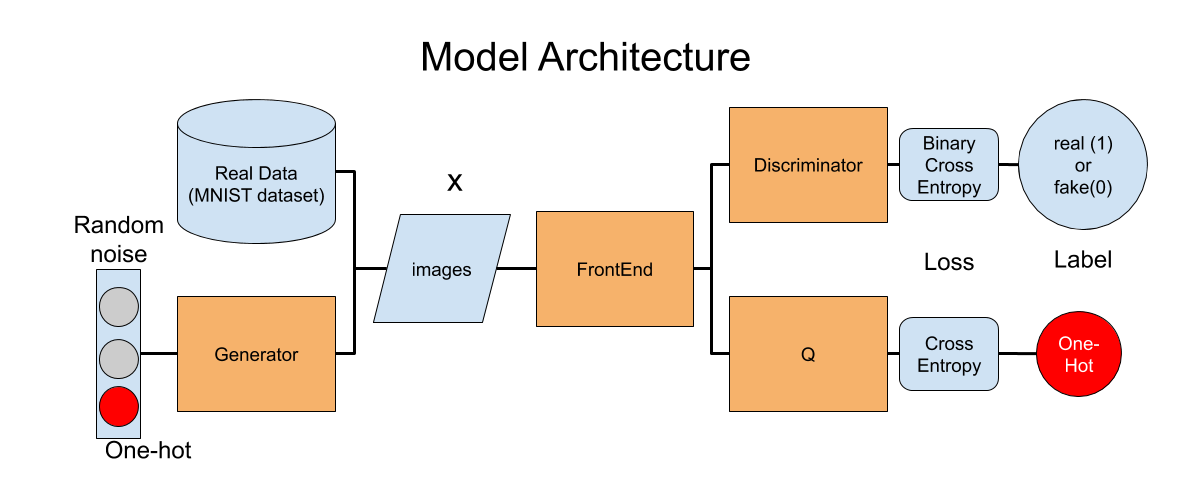
\includegraphics[width=\linewidth]{Images/modelarch.png}
\caption{Architecture of my implement}
\end{figure}

Implement of model architecture as follows :

\begin{minted}[frame=lines, breaklines]{python}
class Generator(nn.Module):
    def __init__(self, noise_size, feature_size):
        super(Generator, self).__init__()
        
        self.main = nn.Sequential(
            
            nn.ConvTranspose2d(noise_size, feature_size*8, 4, 1, bias=False),
            nn.BatchNorm2d(feature_size*8),
            nn.ReLU(True),
            
            nn.ConvTranspose2d(feature_size*8, feature_size*4, 4, 2, 1, bias=False),
            nn.BatchNorm2d(feature_size*4),
            nn.ReLU(True),
            
            nn.ConvTranspose2d(feature_size*4, feature_size*2, 4, 2, 1, bias=False),
            nn.BatchNorm2d(feature_size*2),
            nn.ReLU(True),
            
            nn.ConvTranspose2d(feature_size*2, feature_size*1, 2, 2, 1, bias=False),
            nn.BatchNorm2d(feature_size*1),
            nn.ReLU(True),
            
            nn.ConvTranspose2d(feature_size*1, 1, 1, 1, 1, bias=False),
            nn.Tanh()
            #nn.Sigmoid()
        )
        self.noise_size = noise_size
        
    def forward(self, x):
        return self.main(x)
    
class FrontEnd(nn.Module):
    def __init__(self, feature_size):
        super(FrontEnd, self).__init__()
        
        self.main = nn.Sequential(
            
            nn.Conv2d(1, feature_size*1, 1, 1, 1, bias=False),
            nn.LeakyReLU(0.2, inplace=True),
            
            nn.Conv2d(feature_size*1, feature_size*2, 2, 2, 1, bias=False),
            nn.BatchNorm2d(feature_size*2),
            nn.LeakyReLU(0.2, inplace=True),
            
            nn.Conv2d(feature_size*2, feature_size*4, 4, 2, 1, bias=False),
            nn.BatchNorm2d(feature_size*4),
            nn.LeakyReLU(0.2, inplace=True),
            
            nn.Conv2d(feature_size*4, feature_size*8, 4, 2, 1, bias=False),
            nn.BatchNorm2d(feature_size*8),
            nn.LeakyReLU(0.2, inplace=True)
        )
    
    def forward(self, x):
        return self.main(x)
    
class Discriminator(nn.Module):
    def __init__(self, feature_size):
        super(Discriminator, self).__init__()
        
        self.main = nn.Sequential(
            nn.Conv2d(feature_size*8, 1, 4, 1, bias=False),
            nn.Sigmoid()
        )
        
    def forward(self, x):
        x = self.main(x)
        #return self.main(x).view(-1, 1)
        return x.view(-1,1)
    
class Q(nn.Module):
    def __init__(self, feature_size):
        super(Q, self).__init__()
        
        self.main = nn.Sequential(
            nn.Linear(feature_size*8*4*4, 100, bias=True),
            nn.ReLU(),
            nn.Linear(100, 10, bias=True)
        )
        
    def forward(self, x):
        x = x.view(x.size(0), -1)
        return self.main(x).squeeze()
\end{minted}

And The loss of Q is cross entropy. Implement as follows (also part of previous section) :

\begin{minted}[frame=lines, breaklines]{python}
# Omit .......
                # Generator and Q part
                optim_G.zero_grad()
                
                # fake_x from previous `fake_x = self.generator(z)`
                fe_out = self.front_end(fake_x)
                ad_out = self.discriminator(fe_out)
                
                # criterion_D = nn.BCELoss().cuda()
                label.data.fill_(1.0)
                loss_G_reconstruct = criterion_D(ad_out, label)
                
                c = self.Q(fe_out)
                
                # criterion_Q = nn.CrossEntropyLoss().cuda()
                loss_Q = criterion_Q(c, idx)
                
                loss_G = loss_G_reconstruct + loss_Q
                loss_G.backward()
                
                optim_G.step()
                
                fake_x = self.generator(z)
                fake_out_after = self.discriminator(self.front_end(fake_x.detach()))
# Omit .......
\end{minted}

\subsubsection{Generate noise and image}

When training, I generated different noise with random cluster index which size is batch size. When evaluation or image generated, I generated same noise with ten cluster index from 0 to 9.

\begin{minted}[frame=lines, breaklines]{python}
# Omit .......
    def _noise_eval(self):
        cluster_num = 10
        
        # gen all cluster one hot vectors
        idx = np.arange(cluster_num)
        c = np.zeros((cluster_num, cluster_num))
        c[range(cluster_num), idx] = 1.0
        
        # gen torch (#cluster, #noise, 1, 1) with same noise
        z = torch.cat([
            torch.FloatTensor(1, self.noise_size - cluster_num).uniform_(-1.0, 1.0).expand(cluster_num, self.noise_size - cluster_num), 
            torch.Tensor(c)
        ] , 1).view(-1, self.noise_size, 1, 1)
        
        return z.cuda(), torch.LongTensor(idx).cuda()
        
    def _noise_sample(self, batch_size=None):
        if batch_size is None:
            batch_size = self.batch_size
        # gen condition c
        cluster_num = 10
        idx = np.random.randint(cluster_num, size=batch_size)
        c = np.zeros((batch_size, cluster_num))
        c[range(batch_size), idx] = 1.0
        
        # gen torch (batch, #noise, 1, 1)
        z = torch.cat([
            torch.FloatTensor(batch_size, self.noise_size - cluster_num).uniform_(-1.0, 1.0), 
            torch.Tensor(c)
        ] , 1).view(-1, self.noise_size, 1, 1)
        
        return z.cuda(), torch.LongTensor(idx).cuda()
# Omit .......
\end{minted}

And I generate fixed result with modify random seed in pytorch.

\begin{minted}[frame=lines, breaklines]{python}
# Omit .......
    def evaluation(self, noise_num=10, seed=None):
        
        if seed is None:
            import time
            seed = time.time()
        
        self.generator.eval()
        
        x = []
        torch.manual_seed(seed)
        for i in range(noise_num):
            z, _ = self._noise_eval()
            x.append( self.generator(z) )
        
        x = torch.cat(x, dim=0)
        
        self.generator.train()
        
        return x.detach().cpu()
# Omit .......
\end{minted}

\subsection{Loss function of generator}

According previous implement, my loss of generator as follows:

\begin{equation}
\text{Loss}_{G, Q} = -E_{z\sim P_z(z)}(\log D(G(z; \theta_G); \theta_D) ) - E_{c\sim P_c(c), z' \sim P_{z'}(z')}(\log Q(c| G(z; \theta_G) ;\theta_Q))
\end{equation}

\section{Experimental results}

\subsection{Generated image from sample}

\begin{figure}[H]
\centering
% \includegraphics[width=\linewidth]{path/to/image}
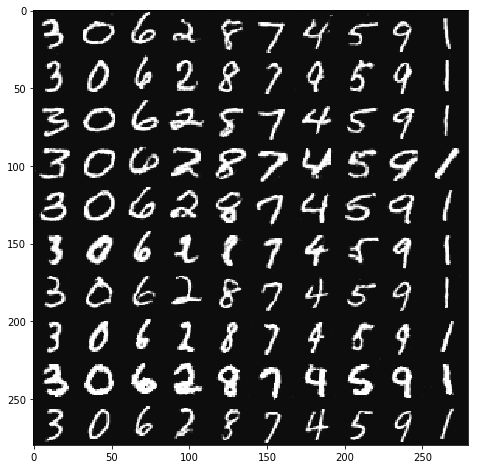
\includegraphics[width=\linewidth]{Images/result.png}
\caption{Result, x-axis is different condition, y-axis is different noise}
\end{figure}

\subsection{Training Loss curve}

\begin{figure}[H]
\centering
% \includegraphics[width=\linewidth]{path/to/image}
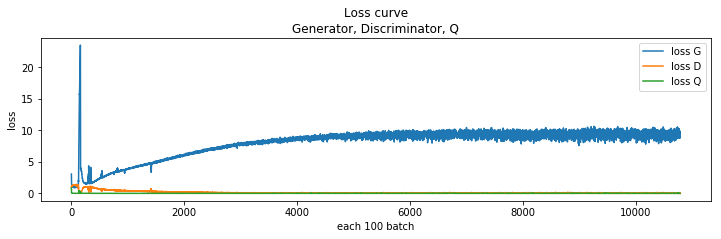
\includegraphics[width=\linewidth]{Images/loss.png}
\caption{Loss curve of Generator, Discriminator, Q}
\end{figure}

\subsection{Training Probability curve}

\begin{figure}[H]
\centering
% \includegraphics[width=\linewidth]{path/to/image}
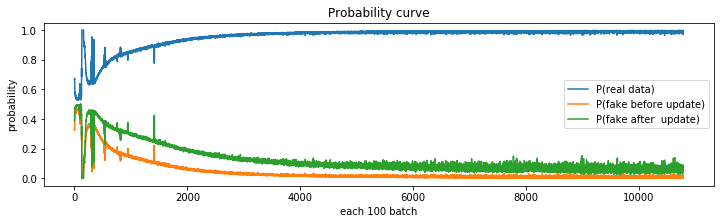
\includegraphics[width=\linewidth]{Images/prob.png}
\caption{Probability of real data, fake data before G updating and fake data after G updating}
\end{figure}

\newpage

\section{Discussion}

\subsection{Broken InfoGAN}

When I does this lab, I find easily get a broken InfoGAN in final. But they looks good in begining. After special point, model usually can't recovery.

\begin{figure}[H]
\centering
% \includegraphics[width=\linewidth]{path/to/image}
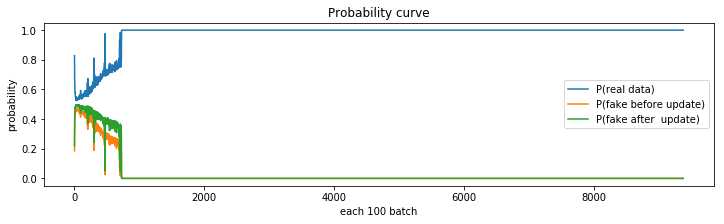
\includegraphics[width=\linewidth]{Images/probbroken.png}
\caption{Probability of real data, fake data before G updating and fake data after G updating}
\end{figure}

I find discriminator became too strong too powerful lead to generator can't adversary discriminator. Because the green line can't greater than orange line after that broken point.

%\begin{figure}[H]
%\centering
% \includegraphics[width=\linewidth]{path/to/image}
%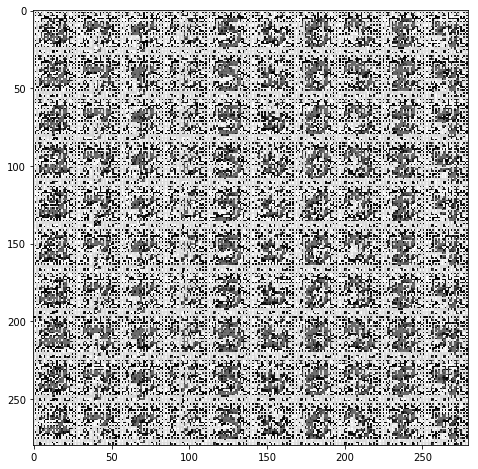
\includegraphics[width=\linewidth]{Images/resultbroken.png}
%\caption{Result, x-axis is different condition, y-axis is different noise}
%\end{figure}

% --------------------------------------------------------------
%     You don't have to mess with anything below this line.
% --------------------------------------------------------------
 
\end{document}